% ============================================================
%  §7  Conclusion
% ============================================================

\section{Conclusion}
\label{sec:conclusion}

This paper has proposed Information Field Geometry Theory (IFGT) and redefined information as the
structure of a quasi-closure that persists as a trace of difference.
Under this framing, information is understood not as a description of states or an independent
substance, but as a geometric structure that constrains the paths and distributions of difference
chains.

IFGT is positioned as an upper-layer theory built upon the generative structure described by
Vortical Enclosure Dynamics (VED), and it clarifies the correspondence between physical persistence
through closure and informational structure through quasi-closure.
The two are not opposing theories but complementary frameworks describing the same generative
structure from different aspects.
In particular, by formulating the relation between information density~$I$ and closure degree~$C$
as $I = f(1-C)$, the division of roles between the two theories is made explicit at the level of
variables.

The theory introduces the information density~$I$, the information flow~$J$, the information
potential~$\Phi$, the informational time~$\tau$, and the generation term~$\sigma$ to describe
motion within a quasi-closure.
In Section~5, $\sigma$ is expanded into three contributions---driving, dissipation, and
barrier---and a single evolution equation for the closure-degree field~$C(x,\tau)$ is obtained as
the unified VED$\times$IFGT equation~(11).
This equation is derived from two minimal axioms: \emph{there is difference} and \emph{difference
tends to close}.

Within this framework, information appears not as a static object of description, but as a dynamic
process that participates in structural formation through the persistence of difference and the
constraint of flow.
Physical structure and informational structure are not separated entities; they are understood as
being generated cyclically through mutual influence.

The scope of the IFGT concept of information relative to existing frameworks is summarized in
Fig.~\ref{fig:coverage_map}: IFGT addresses the full continuum of closure degree~$C$, integrating
the domains covered by Shannon information, affordance, common-sense information, and physical
information into a single dynamical description.

\begin{figure}[h]
  \centering
  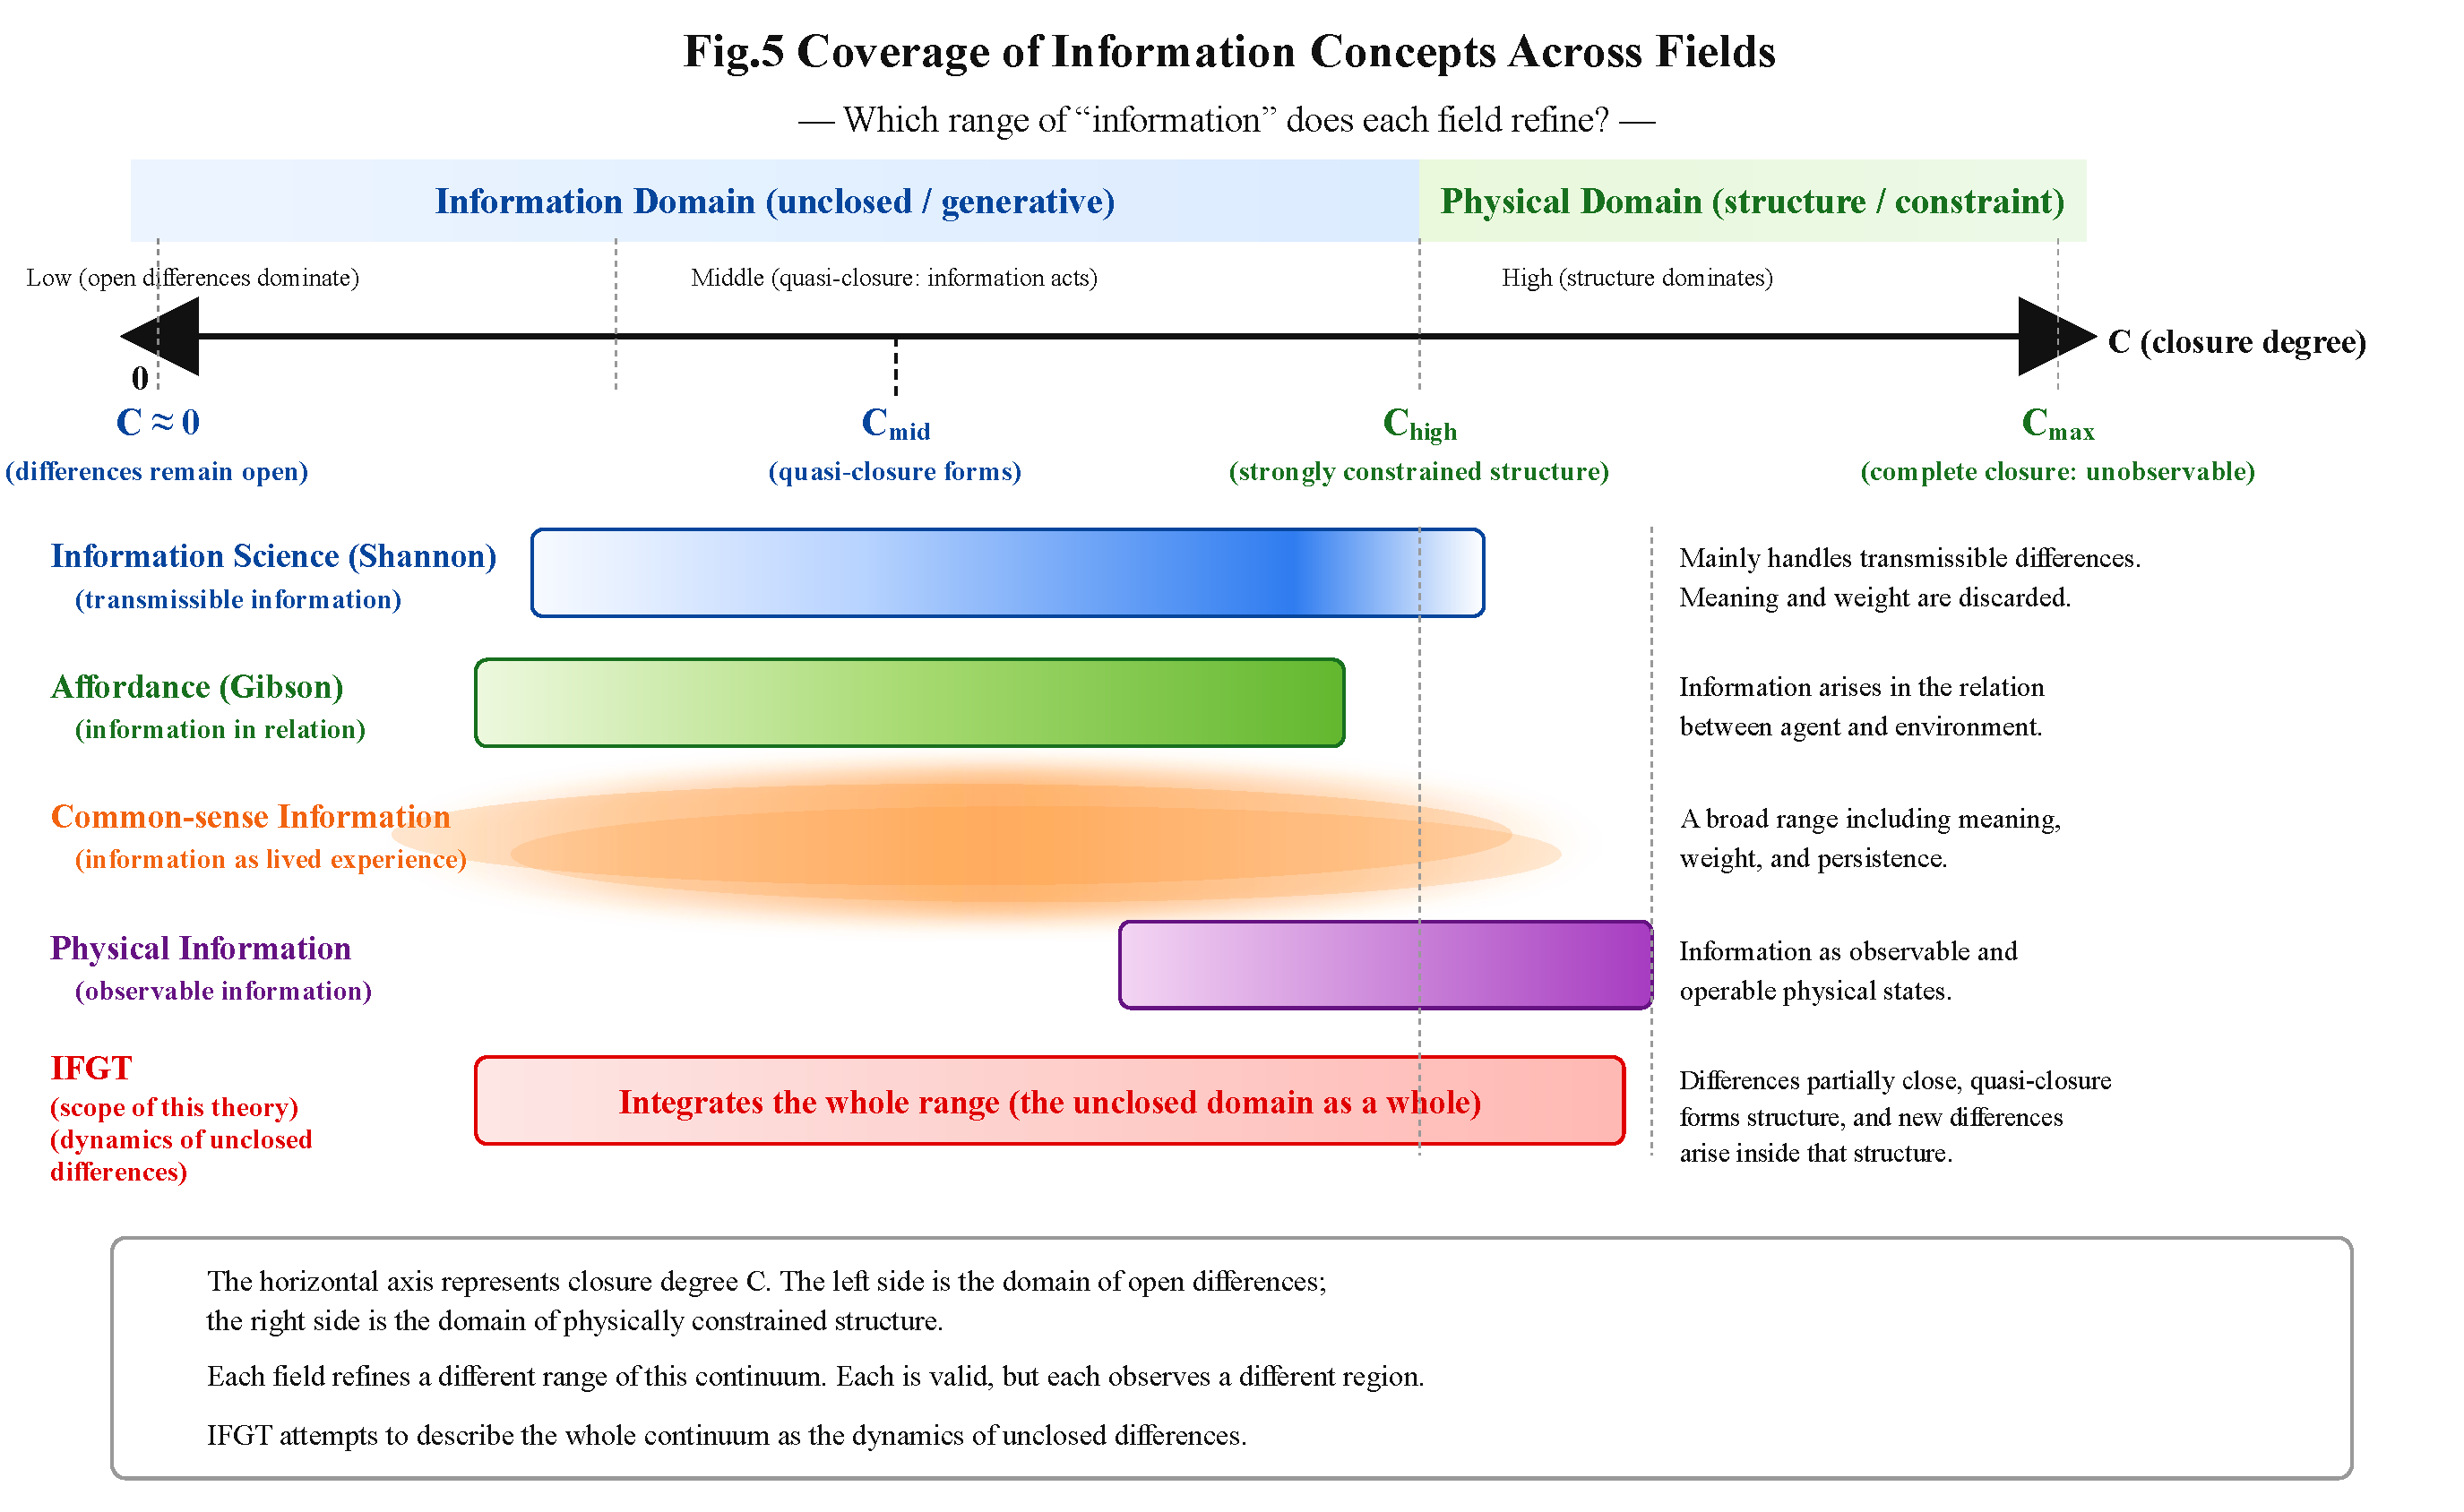
\includegraphics[width=0.92\textwidth]{figures/fig5_information_coverage_map_recreated_en.pdf}
  \caption{Coverage of information concepts across fields.
    The horizontal axis represents closure degree~$C$.
    Each field refines a different range of this continuum.
    IFGT attempts to describe the whole continuum as the dynamics of unclosed differences.}
  \label{fig:coverage_map}
\end{figure}

This paper has not addressed the concrete implementations in biological or computational systems,
but the structure described by IFGT is suggested to appear prominently in such systems.
The theory aims at a general description of structure that does not depend on any particular domain.

The scope of the theory is, at present, limited to the minimal description of informational
structure and the introduction of the unified equation.
Further developments may include the correspondence with concrete structures in domains such as
life, consciousness, language, and intelligence, as well as detailed analysis of the unified
equation~(11) (classification of stable solutions, existence conditions for limit-cycle solutions,
renormalization structure, and so on), but these lie beyond the direct scope of this paper.

In sum, IFGT provides a minimal theory for describing, as geometry, the motion of quasi-closure
that persists in the process by which structure is generated from difference.
This paper presents its foundational framework; detailed developments and applications remain as
future work.
